\documentclass[9pt]{beamer}
\usepackage[utf8]{inputenc}
\usefonttheme{serif} 
\usefonttheme{structuresmallcapsserif} 
\usepackage{hyperref}
\hypersetup{
    colorlinks=true,
    linkcolor=blue,
    filecolor=magenta,
    urlcolor=cyan,
}

\usetheme{Luebeck}
%\usepackage{media9}
%\usepackage{animate}
\usepackage{multimedia}
\usepackage{textpos} 

\addtobeamertemplate{frametitle}{}{%
    \begin{textblock*}{100mm}(11.75cm,-0.86cm)
        
\includegraphics[height=0.86cm,width=0.86cm]{HIPlogo.png}
    \end{textblock*}
    }
\addtobeamertemplate{frametitle}{}{%
    \begin{textblock*}{100mm}(10.89cm,-0.86cm)
        
\includegraphics[height=0.86cm,width=0.86cm]{HYlogo.jpg}
    \end{textblock*}}
\addtobeamertemplate{frametitle}{}{%
    \begin{textblock*}{100mm}(10.03cm,-0.86cm)
        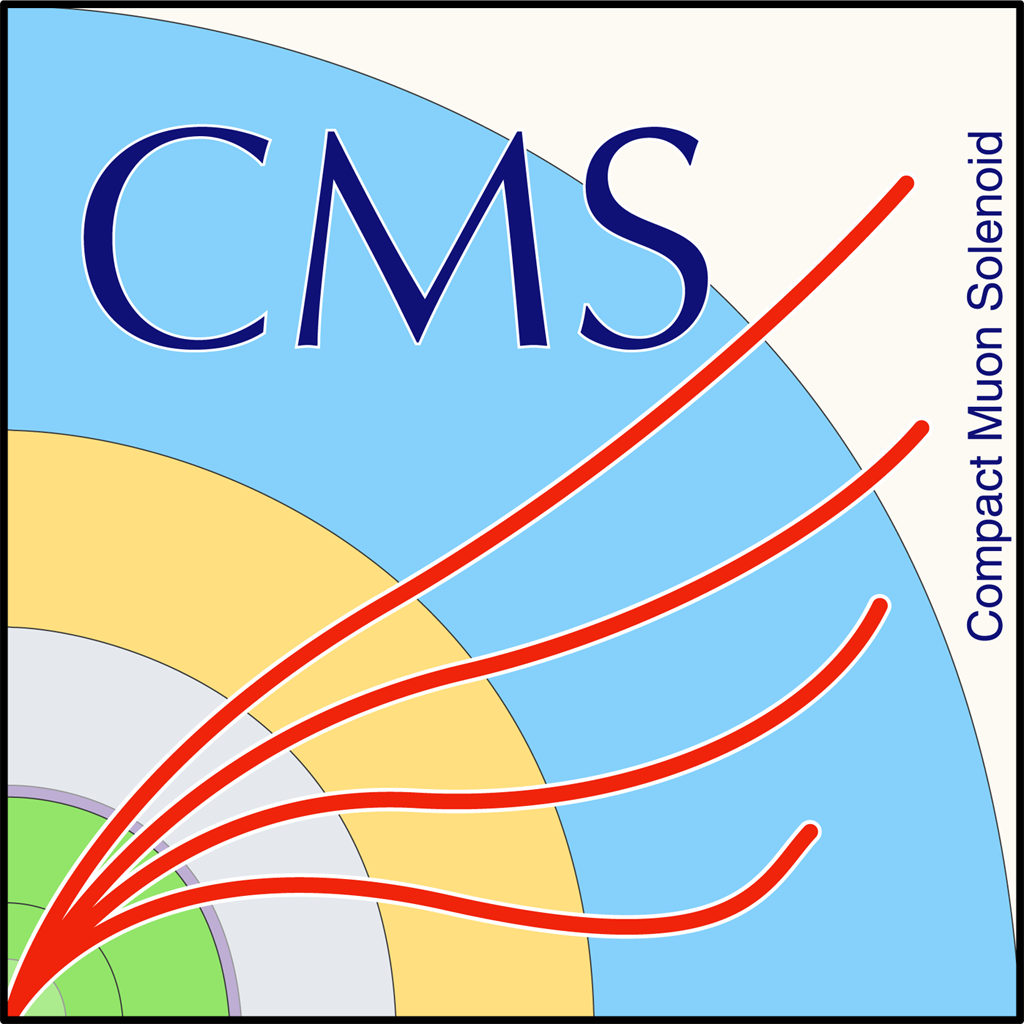
\includegraphics[height=0.86cm,width=0.86cm]{CMSlogo.png}
    \end{textblock*}}

\definecolor{ao}{rgb}{0.0, 0.5, 0.0}
\definecolor{darkgreen}{rgb}{0.0, 0.2, 0.13}
\definecolor{ferngreen}{rgb}{0.31, 0.47, 0.26}
    
\usecolortheme[named=ferngreen]{structure}
\beamertemplatenavigationsymbolsempty
\setbeamertemplate{bibliography item}[text]
\title[BCD16 (Legacy ReReco) hot zones]{BCD16 (Legacy ReReco) hot zones}
%\subtitle{JERC meeting 26th Feb 2018}
\author{Hannu Siikonen}
\institute{Helsinki Institute of Physics \\ \vspace{0.25cm} Instructor Adj.~Prof.~Mikko~Voutilainen}

\date{\today}

\setbeamersize{text margin left=5pt,text margin right=5pt}
\setlength{\labelsep}{12pt}

\begin{document}

\begin{frame}[t]
\titlepage
\end{frame}

\begin{frame}[t]{Motivation}
\begin{itemize}
 \item In the past we have produced histograms for exlcuding ECAL hot zones
 \item More recently, there was a discussion on cleaning certain areas in HCAL \footnote{\url{https://groups.cern.ch/group/CMS-JME-L2L3Residual-Analysts/Lists/Archive/Flat.aspx?RootFolder=\%2fgroup\%2fCMS-JME-L2L3Residual-Analysts\%2fLists\%2fArchive\%2fFollow\%20up\%20on\%20HCAL\%20hot\%20towers\%20cleaning&FolderCTID=0x012002000BA29B1615BA554D933D94B87E1E3AC3}}
 \item In these slides I will present an update of the hot tower analysis (ECAL+HCAL)
 \item Underlying data: $\eta - \phi$ histograms of jet counts for the triggering jet of each HLT\_PFJet\* trigger separately
 \item Definitions:
 \begin{itemize}
 \item Relative fluctuation plots show the fluctuation w.r.t. to the "pedestal", averaged over phi in each eta sector
 \item The excess/deficit plots show the deviation from the pedestal divided by the rms value
 \item From the (final) pedestal averaging and the (final) rms value we exclude values over 2 (initial) rms values away from the (initial) pedestal
 \item The Black patches: The suggested exclusion zones based on combined BCDEF Data
 \item P8M1: the old pythia8 tune
 \item P8CP5: the new pythia8 tune
 \item HS1: the Herwig++ tune
 \end{itemize}
\end{itemize}
\end{frame}

\begin{frame}[t]{HLT\_ZeroBias Njets (Data, P8M1)}
\begin{columns}[T]
  \begin{column}{.5\textwidth}
  \includegraphics[width=\linewidth]{../pdf/dataquality_njet_jt0.pdf}
  \end{column}
  \begin{column}{.5\textwidth}
  \includegraphics[width=\linewidth]{../pdf/mcquality_njet_jt0.pdf}
  \end{column}
\end{columns}
\end{frame}

\begin{frame}[t]{HLT\_ZeroBias Njets (P8M1, HS1)}
\begin{columns}[T]
  \begin{column}{.5\textwidth}
  \includegraphics[width=\linewidth]{../pdf/mcquality_njet_jt0.pdf}
  \end{column}
  \begin{column}{.5\textwidth}
  \includegraphics[width=\linewidth]{../pdf/hwquality_njet_jt0.pdf}
  \end{column}
\end{columns}
\end{frame}

\begin{frame}[t]{HLT\_ZeroBias Data}
\begin{columns}[T]
  \begin{column}{.5\textwidth}
  \includegraphics[width=\linewidth]{../pdf/dataquality_relfluctuation_jt0.pdf}
  \end{column}
  \begin{column}{.5\textwidth}
  \includegraphics[width=\linewidth]{../pdf/dataquality_significance_jt0.pdf}
  \end{column}
\end{columns}
\end{frame}

\begin{frame}[t]{HLT\_ZeroBias HS1}
\begin{columns}[T]
  \begin{column}{.5\textwidth}
  \includegraphics[width=\linewidth]{../pdf/hwquality_relfluctuation_jt0.pdf}
  \end{column}
  \begin{column}{.5\textwidth}
  \includegraphics[width=\linewidth]{../pdf/hwquality_significance_jt0.pdf}
  \end{column}
\end{columns}
\end{frame}

\begin{frame}[t]{HLT\_ZeroBias P8M1}
\begin{columns}[T]
  \begin{column}{.5\textwidth}
  \includegraphics[width=\linewidth]{../pdf/mcquality_relfluctuation_jt0.pdf}
  \end{column}
  \begin{column}{.5\textwidth}
  \includegraphics[width=\linewidth]{../pdf/mcquality_significance_jt0.pdf}
  \end{column}
\end{columns}
\end{frame}


\begin{frame}[t]{HLT\_PFJet40 Njets (Data, P8M1)}
\begin{columns}[T]
  \begin{column}{.5\textwidth}
  \includegraphics[width=\linewidth]{../pdf/dataquality_njet_jt40.pdf}
  \end{column}
  \begin{column}{.5\textwidth}
  \includegraphics[width=\linewidth]{../pdf/mcquality_njet_jt40.pdf}
  \end{column}
\end{columns}
\end{frame}

\begin{frame}[t]{HLT\_PFJet40 Njets (P8M1, HS1)}
\begin{columns}[T]
  \begin{column}{.5\textwidth}
  \includegraphics[width=\linewidth]{../pdf/mcquality_njet_jt40.pdf}
  \end{column}
  \begin{column}{.5\textwidth}
  \includegraphics[width=\linewidth]{../pdf/hwquality_njet_jt40.pdf}
  \end{column}
\end{columns}
\end{frame}

\begin{frame}[t]{HLT\_PFJet40 Data}
\begin{columns}[T]
  \begin{column}{.5\textwidth}
  \includegraphics[width=\linewidth]{../pdf/dataquality_relfluctuation_jt40.pdf}
  \end{column}
  \begin{column}{.5\textwidth}
  \includegraphics[width=\linewidth]{../pdf/dataquality_significance_jt40.pdf}
  \end{column}
\end{columns}
\end{frame}

\begin{frame}[t]{HLT\_PFJet40 HS1}
\begin{columns}[T]
  \begin{column}{.5\textwidth}
  \includegraphics[width=\linewidth]{../pdf/hwquality_relfluctuation_jt40.pdf}
  \end{column}
  \begin{column}{.5\textwidth}
  \includegraphics[width=\linewidth]{../pdf/hwquality_significance_jt40.pdf}
  \end{column}
\end{columns}
\end{frame}

\begin{frame}[t]{HLT\_PFJet40 P8M1}
\begin{columns}[T]
  \begin{column}{.5\textwidth}
  \includegraphics[width=\linewidth]{../pdf/mcquality_relfluctuation_jt40.pdf}
  \end{column}
  \begin{column}{.5\textwidth}
  \includegraphics[width=\linewidth]{../pdf/mcquality_significance_jt40.pdf}
  \end{column}
\end{columns}
\end{frame}


\begin{frame}[t]{HLT\_PFJet60 Njets (Data, P8M1)}
\begin{columns}[T]
  \begin{column}{.5\textwidth}
  \includegraphics[width=\linewidth]{../pdf/dataquality_njet_jt60.pdf}
  \end{column}
  \begin{column}{.5\textwidth}
  \includegraphics[width=\linewidth]{../pdf/mcquality_njet_jt60.pdf}
  \end{column}
\end{columns}
\end{frame}

\begin{frame}[t]{HLT\_PFJet60 Njets (P8M1, HS1)}
\begin{columns}[T]
  \begin{column}{.5\textwidth}
  \includegraphics[width=\linewidth]{../pdf/mcquality_njet_jt60.pdf}
  \end{column}
  \begin{column}{.5\textwidth}
  \includegraphics[width=\linewidth]{../pdf/hwquality_njet_jt60.pdf}
  \end{column}
\end{columns}
\end{frame}

\begin{frame}[t]{HLT\_PFJet60 Data}
\begin{columns}[T]
  \begin{column}{.5\textwidth}
  \includegraphics[width=\linewidth]{../pdf/dataquality_relfluctuation_jt60.pdf}
  \end{column}
  \begin{column}{.5\textwidth}
  \includegraphics[width=\linewidth]{../pdf/dataquality_significance_jt60.pdf}
  \end{column}
\end{columns}
\end{frame}

\begin{frame}[t]{HLT\_PFJet60 HS1}
\begin{columns}[T]
  \begin{column}{.5\textwidth}
  \includegraphics[width=\linewidth]{../pdf/hwquality_relfluctuation_jt60.pdf}
  \end{column}
  \begin{column}{.5\textwidth}
  \includegraphics[width=\linewidth]{../pdf/hwquality_significance_jt60.pdf}
  \end{column}
\end{columns}
\end{frame}

\begin{frame}[t]{HLT\_PFJet60 P8M1}
\begin{columns}[T]
  \begin{column}{.5\textwidth}
  \includegraphics[width=\linewidth]{../pdf/mcquality_relfluctuation_jt60.pdf}
  \end{column}
  \begin{column}{.5\textwidth}
  \includegraphics[width=\linewidth]{../pdf/mcquality_significance_jt60.pdf}
  \end{column}
\end{columns}
\end{frame}


\begin{frame}[t]{HLT\_PFJet80 Njets (Data, P8M1)}
\begin{columns}[T]
  \begin{column}{.5\textwidth}
  \includegraphics[width=\linewidth]{../pdf/dataquality_njet_jt80.pdf}
  \end{column}
  \begin{column}{.5\textwidth}
  \includegraphics[width=\linewidth]{../pdf/mcquality_njet_jt80.pdf}
  \end{column}
\end{columns}
\end{frame}

\begin{frame}[t]{HLT\_PFJet80 Njets (P8M1, HS1)}
\begin{columns}[T]
  \begin{column}{.5\textwidth}
  \includegraphics[width=\linewidth]{../pdf/mcquality_njet_jt80.pdf}
  \end{column}
  \begin{column}{.5\textwidth}
  \includegraphics[width=\linewidth]{../pdf/hwquality_njet_jt80.pdf}
  \end{column}
\end{columns}
\end{frame}

\begin{frame}[t]{HLT\_PFJet80 Data}
\begin{columns}[T]
  \begin{column}{.5\textwidth}
  \includegraphics[width=\linewidth]{../pdf/dataquality_relfluctuation_jt80.pdf}
  \end{column}
  \begin{column}{.5\textwidth}
  \includegraphics[width=\linewidth]{../pdf/dataquality_significance_jt80.pdf}
  \end{column}
\end{columns}
\end{frame}

\begin{frame}[t]{HLT\_PFJet80 HS1}
\begin{columns}[T]
  \begin{column}{.5\textwidth}
  \includegraphics[width=\linewidth]{../pdf/hwquality_relfluctuation_jt80.pdf}
  \end{column}
  \begin{column}{.5\textwidth}
  \includegraphics[width=\linewidth]{../pdf/hwquality_significance_jt80.pdf}
  \end{column}
\end{columns}
\end{frame}

\begin{frame}[t]{HLT\_PFJet80 P8M1}
\begin{columns}[T]
  \begin{column}{.5\textwidth}
  \includegraphics[width=\linewidth]{../pdf/mcquality_relfluctuation_jt80.pdf}
  \end{column}
  \begin{column}{.5\textwidth}
  \includegraphics[width=\linewidth]{../pdf/mcquality_significance_jt80.pdf}
  \end{column}
\end{columns}
\end{frame}


\begin{frame}[t]{HLT\_PFJet140 Njets (Data, P8M1)}
\begin{columns}[T]
  \begin{column}{.5\textwidth}
  \includegraphics[width=\linewidth]{../pdf/dataquality_njet_jt140.pdf}
  \end{column}
  \begin{column}{.5\textwidth}
  \includegraphics[width=\linewidth]{../pdf/mcquality_njet_jt140.pdf}
  \end{column}
\end{columns}
\end{frame}

\begin{frame}[t]{HLT\_PFJet140 Njets (P8M1, HS1)}
\begin{columns}[T]
  \begin{column}{.5\textwidth}
  \includegraphics[width=\linewidth]{../pdf/mcquality_njet_jt140.pdf}
  \end{column}
  \begin{column}{.5\textwidth}
  \includegraphics[width=\linewidth]{../pdf/hwquality_njet_jt140.pdf}
  \end{column}
\end{columns}
\end{frame}

\begin{frame}[t]{HLT\_PFJet140 Data}
\begin{columns}[T]
  \begin{column}{.5\textwidth}
  \includegraphics[width=\linewidth]{../pdf/dataquality_relfluctuation_jt140.pdf}
  \end{column}
  \begin{column}{.5\textwidth}
  \includegraphics[width=\linewidth]{../pdf/dataquality_significance_jt140.pdf}
  \end{column}
\end{columns}
\end{frame}

\begin{frame}[t]{HLT\_PFJet140 HS1}
\begin{columns}[T]
  \begin{column}{.5\textwidth}
  \includegraphics[width=\linewidth]{../pdf/hwquality_relfluctuation_jt140.pdf}
  \end{column}
  \begin{column}{.5\textwidth}
  \includegraphics[width=\linewidth]{../pdf/hwquality_significance_jt140.pdf}
  \end{column}
\end{columns}
\end{frame}

\begin{frame}[t]{HLT\_PFJet140 P8M1}
\begin{columns}[T]
  \begin{column}{.5\textwidth}
  \includegraphics[width=\linewidth]{../pdf/mcquality_relfluctuation_jt140.pdf}
  \end{column}
  \begin{column}{.5\textwidth}
  \includegraphics[width=\linewidth]{../pdf/mcquality_significance_jt140.pdf}
  \end{column}
\end{columns}
\end{frame}


\begin{frame}[t]{HLT\_PFJet200 Njets (Data, P8M1)}
\begin{columns}[T]
  \begin{column}{.5\textwidth}
  \includegraphics[width=\linewidth]{../pdf/dataquality_njet_jt200.pdf}
  \end{column}
  \begin{column}{.5\textwidth}
  \includegraphics[width=\linewidth]{../pdf/mcquality_njet_jt200.pdf}
  \end{column}
\end{columns}
\end{frame}

\begin{frame}[t]{HLT\_PFJet200 Njets (P8M1, HS1)}
\begin{columns}[T]
  \begin{column}{.5\textwidth}
  \includegraphics[width=\linewidth]{../pdf/mcquality_njet_jt200.pdf}
  \end{column}
  \begin{column}{.5\textwidth}
  \includegraphics[width=\linewidth]{../pdf/hwquality_njet_jt200.pdf}
  \end{column}
\end{columns}
\end{frame}

\begin{frame}[t]{HLT\_PFJet200 Data}
\begin{columns}[T]
  \begin{column}{.5\textwidth}
  \includegraphics[width=\linewidth]{../pdf/dataquality_relfluctuation_jt200.pdf}
  \end{column}
  \begin{column}{.5\textwidth}
  \includegraphics[width=\linewidth]{../pdf/dataquality_significance_jt200.pdf}
  \end{column}
\end{columns}
\end{frame}

\begin{frame}[t]{HLT\_PFJet200 HS1}
\begin{columns}[T]
  \begin{column}{.5\textwidth}
  \includegraphics[width=\linewidth]{../pdf/hwquality_relfluctuation_jt200.pdf}
  \end{column}
  \begin{column}{.5\textwidth}
  \includegraphics[width=\linewidth]{../pdf/hwquality_significance_jt200.pdf}
  \end{column}
\end{columns}
\end{frame}

\begin{frame}[t]{HLT\_PFJet200 P8M1}
\begin{columns}[T]
  \begin{column}{.5\textwidth}
  \includegraphics[width=\linewidth]{../pdf/mcquality_relfluctuation_jt200.pdf}
  \end{column}
  \begin{column}{.5\textwidth}
  \includegraphics[width=\linewidth]{../pdf/mcquality_significance_jt200.pdf}
  \end{column}
\end{columns}
\end{frame}


\begin{frame}[t]{HLT\_PFJet260 Njets (Data, P8M1)}
\begin{columns}[T]
  \begin{column}{.5\textwidth}
  \includegraphics[width=\linewidth]{../pdf/dataquality_njet_jt260.pdf}
  \end{column}
  \begin{column}{.5\textwidth}
  \includegraphics[width=\linewidth]{../pdf/mcquality_njet_jt260.pdf}
  \end{column}
\end{columns}
\end{frame}

\begin{frame}[t]{HLT\_PFJet260 Njets (P8M1, HS1)}
\begin{columns}[T]
  \begin{column}{.5\textwidth}
  \includegraphics[width=\linewidth]{../pdf/mcquality_njet_jt260.pdf}
  \end{column}
  \begin{column}{.5\textwidth}
  \includegraphics[width=\linewidth]{../pdf/hwquality_njet_jt260.pdf}
  \end{column}
\end{columns}
\end{frame}

\begin{frame}[t]{HLT\_PFJet260 Data}
\begin{columns}[T]
  \begin{column}{.5\textwidth}
  \includegraphics[width=\linewidth]{../pdf/dataquality_relfluctuation_jt260.pdf}
  \end{column}
  \begin{column}{.5\textwidth}
  \includegraphics[width=\linewidth]{../pdf/dataquality_significance_jt260.pdf}
  \end{column}
\end{columns}
\end{frame}

\begin{frame}[t]{HLT\_PFJet260 HS1}
\begin{columns}[T]
  \begin{column}{.5\textwidth}
  \includegraphics[width=\linewidth]{../pdf/hwquality_relfluctuation_jt260.pdf}
  \end{column}
  \begin{column}{.5\textwidth}
  \includegraphics[width=\linewidth]{../pdf/hwquality_significance_jt260.pdf}
  \end{column}
\end{columns}
\end{frame}

\begin{frame}[t]{HLT\_PFJet260 P8M1}
\begin{columns}[T]
  \begin{column}{.5\textwidth}
  \includegraphics[width=\linewidth]{../pdf/mcquality_relfluctuation_jt260.pdf}
  \end{column}
  \begin{column}{.5\textwidth}
  \includegraphics[width=\linewidth]{../pdf/mcquality_significance_jt260.pdf}
  \end{column}
\end{columns}
\end{frame}


\begin{frame}[t]{HLT\_PFJet320 Njets (Data, P8M1)}
\begin{columns}[T]
  \begin{column}{.5\textwidth}
  \includegraphics[width=\linewidth]{../pdf/dataquality_njet_jt320.pdf}
  \end{column}
  \begin{column}{.5\textwidth}
  \includegraphics[width=\linewidth]{../pdf/mcquality_njet_jt320.pdf}
  \end{column}
\end{columns}
\end{frame}

\begin{frame}[t]{HLT\_PFJet320 Njets (P8M1, HS1)}
\begin{columns}[T]
  \begin{column}{.5\textwidth}
  \includegraphics[width=\linewidth]{../pdf/mcquality_njet_jt320.pdf}
  \end{column}
  \begin{column}{.5\textwidth}
  \includegraphics[width=\linewidth]{../pdf/hwquality_njet_jt320.pdf}
  \end{column}
\end{columns}
\end{frame}

\begin{frame}[t]{HLT\_PFJet320 Data}
\begin{columns}[T]
  \begin{column}{.5\textwidth}
  \includegraphics[width=\linewidth]{../pdf/dataquality_relfluctuation_jt320.pdf}
  \end{column}
  \begin{column}{.5\textwidth}
  \includegraphics[width=\linewidth]{../pdf/dataquality_significance_jt320.pdf}
  \end{column}
\end{columns}
\end{frame}

\begin{frame}[t]{HLT\_PFJet320 HS1}
\begin{columns}[T]
  \begin{column}{.5\textwidth}
  \includegraphics[width=\linewidth]{../pdf/hwquality_relfluctuation_jt320.pdf}
  \end{column}
  \begin{column}{.5\textwidth}
  \includegraphics[width=\linewidth]{../pdf/hwquality_significance_jt320.pdf}
  \end{column}
\end{columns}
\end{frame}

\begin{frame}[t]{HLT\_PFJet320 P8M1}
\begin{columns}[T]
  \begin{column}{.5\textwidth}
  \includegraphics[width=\linewidth]{../pdf/mcquality_relfluctuation_jt320.pdf}
  \end{column}
  \begin{column}{.5\textwidth}
  \includegraphics[width=\linewidth]{../pdf/mcquality_significance_jt320.pdf}
  \end{column}
\end{columns}
\end{frame}


\begin{frame}[t]{HLT\_PFJet400 Njets (Data, P8M1)}
\begin{columns}[T]
  \begin{column}{.5\textwidth}
  \includegraphics[width=\linewidth]{../pdf/dataquality_njet_jt400.pdf}
  \end{column}
  \begin{column}{.5\textwidth}
  \includegraphics[width=\linewidth]{../pdf/mcquality_njet_jt400.pdf}
  \end{column}
\end{columns}
\end{frame}

\begin{frame}[t]{HLT\_PFJet400 Njets (P8M1, HS1)}
\begin{columns}[T]
  \begin{column}{.5\textwidth}
  \includegraphics[width=\linewidth]{../pdf/mcquality_njet_jt400.pdf}
  \end{column}
  \begin{column}{.5\textwidth}
  \includegraphics[width=\linewidth]{../pdf/hwquality_njet_jt400.pdf}
  \end{column}
\end{columns}
\end{frame}

\begin{frame}[t]{HLT\_PFJet400 Data}
\begin{columns}[T]
  \begin{column}{.5\textwidth}
  \includegraphics[width=\linewidth]{../pdf/dataquality_relfluctuation_jt400.pdf}
  \end{column}
  \begin{column}{.5\textwidth}
  \includegraphics[width=\linewidth]{../pdf/dataquality_significance_jt400.pdf}
  \end{column}
\end{columns}
\end{frame}

\begin{frame}[t]{HLT\_PFJet400 HS1}
\begin{columns}[T]
  \begin{column}{.5\textwidth}
  \includegraphics[width=\linewidth]{../pdf/hwquality_relfluctuation_jt400.pdf}
  \end{column}
  \begin{column}{.5\textwidth}
  \includegraphics[width=\linewidth]{../pdf/hwquality_significance_jt400.pdf}
  \end{column}
\end{columns}
\end{frame}

\begin{frame}[t]{HLT\_PFJet400 P8M1}
\begin{columns}[T]
  \begin{column}{.5\textwidth}
  \includegraphics[width=\linewidth]{../pdf/mcquality_relfluctuation_jt400.pdf}
  \end{column}
  \begin{column}{.5\textwidth}
  \includegraphics[width=\linewidth]{../pdf/mcquality_significance_jt400.pdf}
  \end{column}
\end{columns}
\end{frame}

\begin{frame}[t]{HLT\_PFJet450 Njets (Data, P8M1)}
\begin{columns}[T]
  \begin{column}{.5\textwidth}
  \includegraphics[width=\linewidth]{../pdf/dataquality_njet_jt450.pdf}
  \end{column}
  \begin{column}{.5\textwidth}
  \includegraphics[width=\linewidth]{../pdf/mcquality_njet_jt450.pdf}
  \end{column}
\end{columns}
\end{frame}

\begin{frame}[t]{HLT\_PFJet450 Njets (P8M1, HS1)}
\begin{columns}[T]
  \begin{column}{.5\textwidth}
  \includegraphics[width=\linewidth]{../pdf/mcquality_njet_jt450.pdf}
  \end{column}
  \begin{column}{.5\textwidth}
  \includegraphics[width=\linewidth]{../pdf/hwquality_njet_jt450.pdf}
  \end{column}
\end{columns}
\end{frame}

\begin{frame}[t]{HLT\_PFJet450 Data}
\begin{columns}[T]
  \begin{column}{.5\textwidth}
  \includegraphics[width=\linewidth]{../pdf/dataquality_relfluctuation_jt450.pdf}
  \end{column}
  \begin{column}{.5\textwidth}
  \includegraphics[width=\linewidth]{../pdf/dataquality_significance_jt450.pdf}
  \end{column}
\end{columns}
\end{frame}

\begin{frame}[t]{HLT\_PFJet450 HS1}
\begin{columns}[T]
  \begin{column}{.5\textwidth}
  \includegraphics[width=\linewidth]{../pdf/hwquality_relfluctuation_jt450.pdf}
  \end{column}
  \begin{column}{.5\textwidth}
  \includegraphics[width=\linewidth]{../pdf/hwquality_significance_jt450.pdf}
  \end{column}
\end{columns}
\end{frame}

\begin{frame}[t]{HLT\_PFJet450 P8M1}
\begin{columns}[T]
  \begin{column}{.5\textwidth}
  \includegraphics[width=\linewidth]{../pdf/mcquality_relfluctuation_jt450.pdf}
  \end{column}
  \begin{column}{.5\textwidth}
  \includegraphics[width=\linewidth]{../pdf/mcquality_significance_jt450.pdf}
  \end{column}
\end{columns}
\end{frame}


%\begin{frame}[t]{HLT\_PFJet500 Njets (Data, P8M1)}
%\begin{columns}[T]
%  \begin{column}{.5\textwidth}
%  \includegraphics[width=\linewidth]{../pdf/dataquality_njet_jt500.pdf}
%  \end{column}
%  \begin{column}{.5\textwidth}
%  \includegraphics[width=\linewidth]{../pdf/mcquality_njet_jt500.pdf}
%  \end{column}
%\end{columns}
%\end{frame}
%
%\begin{frame}[t]{HLT\_PFJet500 Njets (P8M1, HS1)}
%\begin{columns}[T]
%  \begin{column}{.5\textwidth}
%  \includegraphics[width=\linewidth]{../pdf/mcquality_njet_jt500.pdf}
%  \end{column}
%  \begin{column}{.5\textwidth}
%  \includegraphics[width=\linewidth]{../pdf/hwquality_njet_jt500.pdf}
%  \end{column}
%\end{columns}
%\end{frame}
%
%\begin{frame}[t]{HLT\_PFJet500 Data}
%\begin{columns}[T]
%  \begin{column}{.5\textwidth}
%  \includegraphics[width=\linewidth]{../pdf/dataquality_relfluctuation_jt500.pdf}
%  \end{column}
%  \begin{column}{.5\textwidth}
%  \includegraphics[width=\linewidth]{../pdf/dataquality_significance_jt500.pdf}
%  \end{column}
%\end{columns}
%\end{frame}

%\begin{frame}[t]{HLT\_PFJet500 HS1}
%\begin{columns}[T]
%  \begin{column}{.5\textwidth}
%  \includegraphics[width=\linewidth]{../pdf/hwquality_relfluctuation_jt500.pdf}
%  \end{column}
%  \begin{column}{.5\textwidth}
%  \includegraphics[width=\linewidth]{../pdf/hwquality_significance_jt500.pdf}
%  \end{column}
%\end{columns}
%\end{frame}
%
%\begin{frame}[t]{HLT\_PFJet500 P8M1}
%\begin{columns}[T]
%  \begin{column}{.5\textwidth}
%  \includegraphics[width=\linewidth]{../pdf/mcquality_relfluctuation_jt500.pdf}
%  \end{column}
%  \begin{column}{.5\textwidth}
%  \includegraphics[width=\linewidth]{../pdf/mcquality_significance_jt500.pdf}
%  \end{column}
%\end{columns}
%\end{frame}


\begin{frame}[t]{Cumulative summary (Data,P8M1)}
\begin{columns}[T]
  \begin{column}{.5\textwidth}
  \includegraphics[width=\linewidth]{../pdf/dataquality_cumulation.pdf}
  \end{column}
  \begin{column}{.5\textwidth}
  \includegraphics[width=\linewidth]{../pdf/mcquality_cumulation.pdf}
  \end{column}
\end{columns}
\begin{itemize}
 \item Cumulative summary plots over all triggers - attempt to present the excess/deficit plots cumulated over all triggers
 \item In the $\eta$ border zones only the triggers with a sufficient amount of data is used
\end{itemize}
\end{frame}

\begin{frame}[t]{Cumulative summary (P8M1,HS1)}
\begin{columns}[T]
  \begin{column}{.5\textwidth}
  \includegraphics[width=\linewidth]{../pdf/mcquality_cumulation.pdf}
  \end{column}
  \begin{column}{.5\textwidth}
  \includegraphics[width=\linewidth]{../pdf/hwquality_cumulation.pdf}
  \end{column}
\end{columns}
\begin{itemize}
 \item Cumulative summary plots over all triggers - attempt to present the excess/deficit plots cumulated over all triggers
 \item In the $\eta$ border zones only the triggers with a sufficient amount of data is used
\end{itemize}
\end{frame}

\begin{frame}[t]{Filtered cumulative summary Data (hot, cold)}
\begin{columns}[T]
  \begin{column}{.5\textwidth}
  \includegraphics[width=\linewidth]{../pdf/dataquality_hots.pdf}
  \end{column}
  \begin{column}{.5\textwidth}
  \includegraphics[width=\linewidth]{../pdf/dataquality_colds.pdf}
  \end{column}
\end{columns}
\begin{itemize}
 \item The same procedure as on the previous slide, but now we emphasize noise that is significant in more than only one trigger
 \item Hot and cold zones separated
\end{itemize}
\end{frame}

\begin{frame}[t]{Filtered cumulative summary HS1 (hot, cold)}
\begin{columns}[T]
  \begin{column}{.5\textwidth}
  \includegraphics[width=\linewidth]{../pdf/hwquality_hots.pdf}
  \end{column}
  \begin{column}{.5\textwidth}
  \includegraphics[width=\linewidth]{../pdf/hwquality_colds.pdf}
  \end{column}
\end{columns}
\begin{itemize}
 \item The same procedure as on the previous slide, but now we emphasize noise that is significant in more than only one trigger
 \item Hot and cold zones separated
\end{itemize}
\end{frame}

\begin{frame}[t]{Filtered cumulative summary P8M1 (hot, cold)}
\begin{columns}[T]
  \begin{column}{.5\textwidth}
  \includegraphics[width=\linewidth]{../pdf/mcquality_hots.pdf}
  \end{column}
  \begin{column}{.5\textwidth}
  \includegraphics[width=\linewidth]{../pdf/mcquality_colds.pdf}
  \end{column}
\end{columns}
\begin{itemize}
 \item The same procedure as on the previous slide, but now we emphasize noise that is significant in more than only one trigger
 \item Hot and cold zones separated
\end{itemize}
\end{frame}

\end{document}
